\documentclass{beamer}
\usepackage[english, serbian]{babel}

\usepackage{booktabs}
\usepackage{xcolor}
\usepackage{graphicx}

\mode<presentation>
{
    \usetheme{Darmstadt}      % or try Darmstadt, Madrid, Warsaw, ...
	\usecolortheme{default} % or try albatross, beaver, crane, ...
	\usefonttheme{default}  % or try serif, structurebold, ...
	\setbeamertemplate{navigation symbols}{}
	\setbeamertemplate{caption}[numbered]
}

\setbeamertemplate{footline}[frame number] 

\definecolor{cc-blue}{HTML}{1f77b4}
\definecolor{cc-orange}{HTML}{ff7f0e}
\definecolor{cc-green}{HTML}{2ca02c}
\definecolor{cc-red}{HTML}{d62728}
\definecolor{cc-purple}{HTML}{9467bd}

\title[]{Revizori sistema za prepoznavanje lica -- etička pitanja\\\small{Prezentacija u okviru kursa\\računarstvo i društvo\\Matematički fakultet}}
\author{Kosta Grujčić\\mi17012@alas.matf.bg.ac.rs}
\date{}

\begin{document}
	\begin{frame}
		\titlepage
	\end{frame}

	\begin{frame}{Uvod}
		\begin{itemize}
			\item Tehnologija analize lica (eng. \textit{FPT}).
			\bigskip
			\item FPT sistemi su vrlo ranjivi i diskriminišu manjinske grupe.
			\bigskip
			\item Rizik je veći time što kompanije naplaćuju svoje usluge državnim ili privatnim licima.
		\end{itemize}
	\end{frame}

	\begin{frame}
		\begin{itemize}
			\item Algoritamska revizija je vršena kroz pet \textit{etičkih pitanja}.
			\bigskip
			\item Etička pitanja su podeljena na preglede dizajna i etičke konflikte.
		\end{itemize}
	\end{frame}

	\begin{frame}{CelebSET}
		\begin{itemize}
			\item Predstavlja podskup IMDB-WIKI skupa podataka.
			\bigskip
			\item Sadrži 80 identita poznatih ličnosti podeljenih u 4 grupe.
			\bigskip
			\item Prevazilaženje postojećih nedostataka algoritamske revizije.
		\end{itemize}
	\end{frame}

	\begin{frame}{Metodologija}
		\begin{itemize}
			\item Porede se rešenja Microsot-a, Amazon-a i Clarifai-a.
			\bigskip
			\item Poređenje se vrši na problemima:
			\begin{itemize}
				\item prepoznavanja pola
				\item identifikovanja imena
				\item određivanje uzrasta
			\end{itemize}
		\end{itemize}
	\end{frame}

	\begin{frame}{Statistika}
		\begin{table}[h!]
			\centering
			\caption{\textbf{Sveukupne performanse na odabranim problemima predviđanja karakteristika lica.}}
			\begin{tabular}{c|ccccc} \toprule
				{} & {Pol} & {Uzrast} & {Ime} & {Osmeh} & {Detekcija} \\ \midrule
				{Microsft} & 99.94\% & 74.09\% & 98.69\% & 79.94\% & 93.56\% \\ 
				{Amazon} & 99.75\% & 58.40\% & 87.25\% & 94.16\% & 99.25\% \\
				{Clarifai} & 85.97\% & 55.24\% & 95.00\% & 56.19\% & 99.31\%\\ \bottomrule
			\end{tabular}
		\end{table}
	\end{frame}

	\begin{frame}
		\begin{table}[h!]
			\centering
			\caption{\textbf{Razlika uspešnosti na subjektima svetlije (L) i tamnije (D) boje kože.}}
			\begin{tabular}{c|ccccc} \toprule
				{} & {Pol} & {Uzrast} & {Ime} & {Osmeh} & {Detekcija} \\ \midrule
				{Microsft} & 0.13\% & 18.35\% & 1.41\% & -0.48\% & 3.38\% \\ 
				{Amazon} & 0.25\% & 16.83\% & 1.03\% & -0.75\% & 0.25\% \\
				{Clarifai} & 11.69\% & 1.00\% & 7.50\% & 0.12\% & 0.42\%\\ \bottomrule
			\end{tabular}
			\label{table:unitary-color}
		\end{table}
	\end{frame}

	\begin{frame}
		\begin{table}[h!]
			\centering
			\caption{\textbf{Razlika uspešnosti na subjektima muškog (M) i ženskog (F) pola.}}
			\begin{tabular}{c|ccccc} \toprule
				{} & {Pol} & {Uzrast} & {Ime} & {Osmeh} & {Detekcija} \\ \midrule
				{Microsft} & 0.13\% & 9.90\% & 1.23\% & -4.45\% & 0.62\% \\ 
				{Amazon} & 0.00\% & 12.28\% & 4.75\% & -9.00\% & 0.50\% \\
				{Clarifai} & 7.58\% & 10.26\% & -1.01\% & 1.25\% & -1.63\%\\ \bottomrule
			\end{tabular}
			\label{table:unitary-gender}
		\end{table}
	\end{frame}

	\begin{frame}{Pregledi dizajna}
		\begin{itemize}
			\item Pregled 1: Definisanje opsega delovanja
			\bigskip
			\item Pregled 2: Revizija zarad pravičnosti postupka
		\end{itemize}
	\end{frame}

	\begin{frame}{Etički konflikti}
		\begin{itemize}
			\item Konflikt 1: Privanost i zastupljenost
			\bigskip
			\item Konflikt 2: Intersekcionalna i grupna jednakost
			\bigskip
			\item Konflikt 3: Transparentnost i prekomerna izloženost		
		\end{itemize}
	\end{frame}

	\begin{frame}
		\begin{table}[h!]
			\centering				
				\caption{\textbf{Udeo etničkih grupa u IMDB-WIKI skupu podataka.}}
				\resizebox{\linewidth}{!}{%
				\begin{tabular}{c|cccccccc} \toprule
					{} & {Azijati} & {Belci} & {Hispano} & {Crnci} & {Arapi} & {Indijci} & {Ostalo} & {Ukupno} \\ \midrule
					{IMDB-WIKI} & 7,557 & 338,896 & 351 & 29,613 & 1,160 & 3,299 & 33,468 & 414,344 \\
					{} & 1.8\% & 81.8\% & 0.1\% & 7.2\% & 0.3\% & 0.8\% & 8.1\% & 100.0\% \\ \bottomrule
				\end{tabular}}
				\label{table:ethnicity-imdb-wiki}
		\end{table}
	\end{frame}
	
	\begin{frame}
		\begin{table}[h!]
			\centering
			\caption{\textbf{Udeo polova u IMDB-WIKI skupu podataka.}}
			\begin{tabular}{ccccc} \toprule
				{} & {Muškarci} & {Žene} & {Nepoznato} & {Ukupno} \\ \midrule
				{IMDB-WIKI} & 230,912 & 179,900 & 3,532 & 414,344 \\
				{} & 55.7\% & 43.4\% & 0.85\% & 100\% \\ \bottomrule
			\end{tabular}
			\label{table:gender-imdb-wiki}
		\end{table}
	\end{frame}

	\begin{frame}
		\begin{figure}[h!]
			\centerline{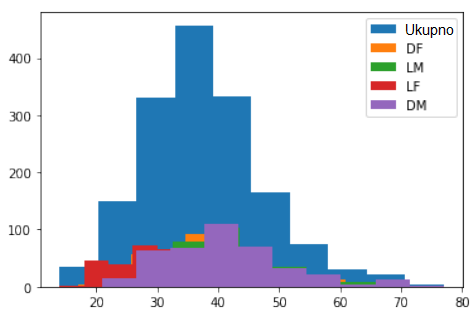
\includegraphics[width=0.65\linewidth]{hist.PNG}}
			\caption{\textbf{Histogram raspodele uzrasta u CelebSET-u. Medijana je 37, moda 36 a srednja vrednost 37.56. Najmlađa osoba ima 14 godina, dok najstarija ima 77. \textcolor{cc-purple}{Ljubičasta}, \textcolor{cc-orange}{narandžasta}, \textcolor{cc-green}{zelena} i \textcolor{cc-red}{crvena} odgovaraju raspodeli uzrasta redom crncima, belcima, crnkinjama i belkinjama.}}
		\end{figure}
	\end{frame}

	\begin{frame}{Rezultati algoritamske revizije}
		\begin{itemize}
			\item CelebSET treba koristiti cilju zastoja ili prekida razvoja, ali ne i kao preduslov za uvođenje moratorijuma.
			\bigskip
			\item Uspeh na CelebSET-u ne treba shvatiti kao vrlo nizak prag koji se mora ispoštovati.
		\end{itemize}
	\end{frame}

	\begin{frame}{Zaključak}
		\begin{itemize}
			\item Tokom kreiranja CelebSET- uočeno je nekoliko etičkih prestupa.
			\bigskip
			\item Standardizovana je algortamska revizija.
			\bigskip
			\item Proces revizije mora imati pažljivo razmotreno pitanje privatnosti.
		\end{itemize}
	\end{frame}
\end{document}